\chapter{Appendix}

\section{Example Images}

\begin{figure}[!htb]
\minipage{0.32\textwidth}
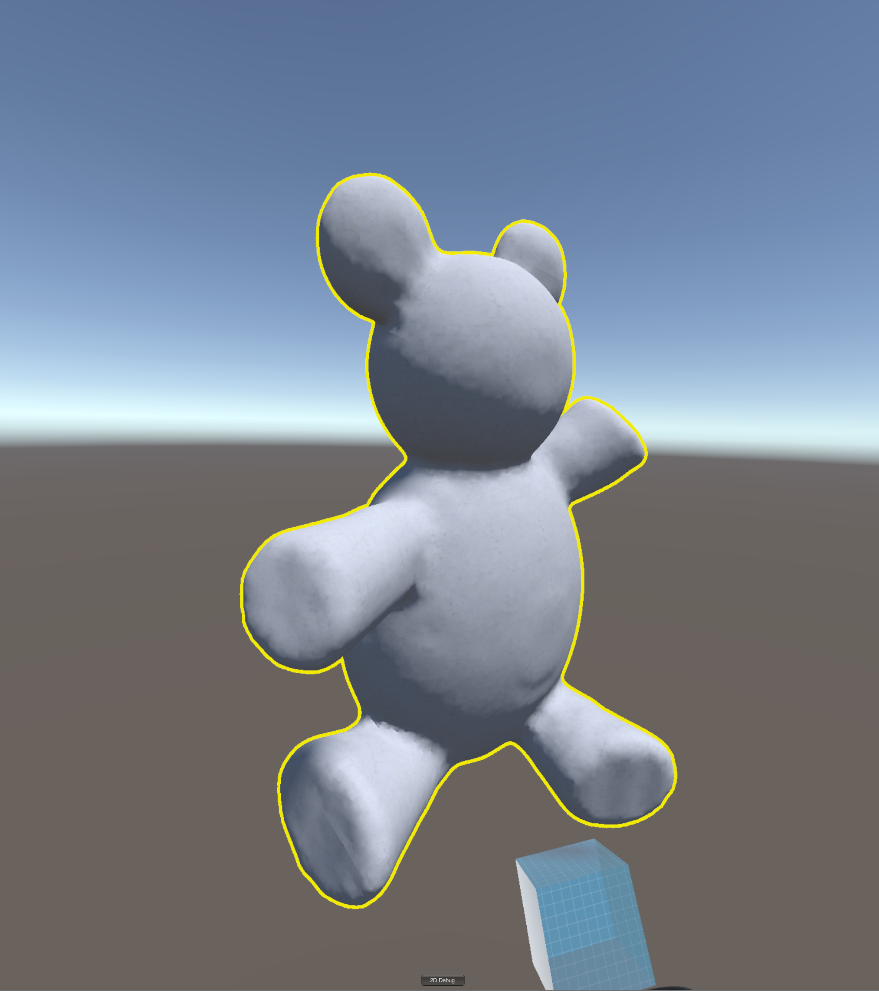
\includegraphics[width=\linewidth]{sculpting_before_edit.png}
\caption{A query result 3D model that has been voxelized into a sculpture.}
\label{fig:sculpting_before_edit}
\endminipage\hfill
\minipage{0.32\textwidth}
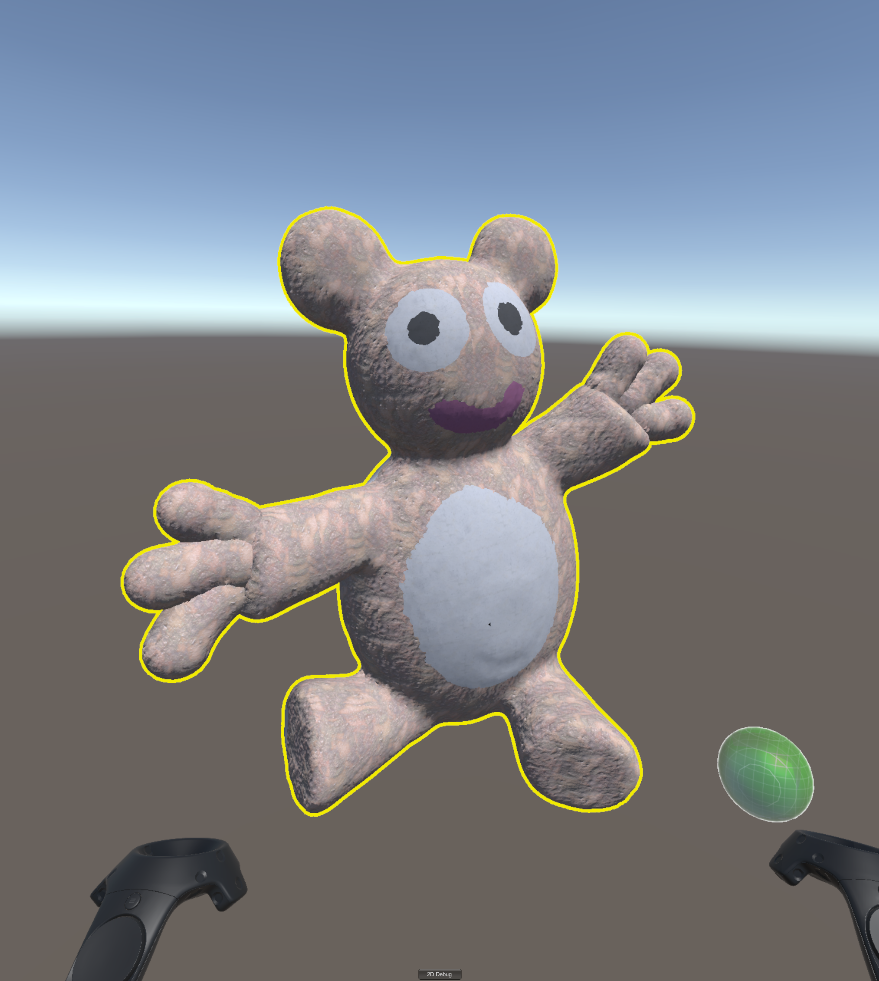
\includegraphics[width=\linewidth]{sculpting_after_edit.png}
\caption{The same sculpture from \ref{fig:sculpting_before_edit} but after several edits.}
\label{fig:sculpting_after_edit}
\endminipage\hfill
\minipage{0.32\textwidth}
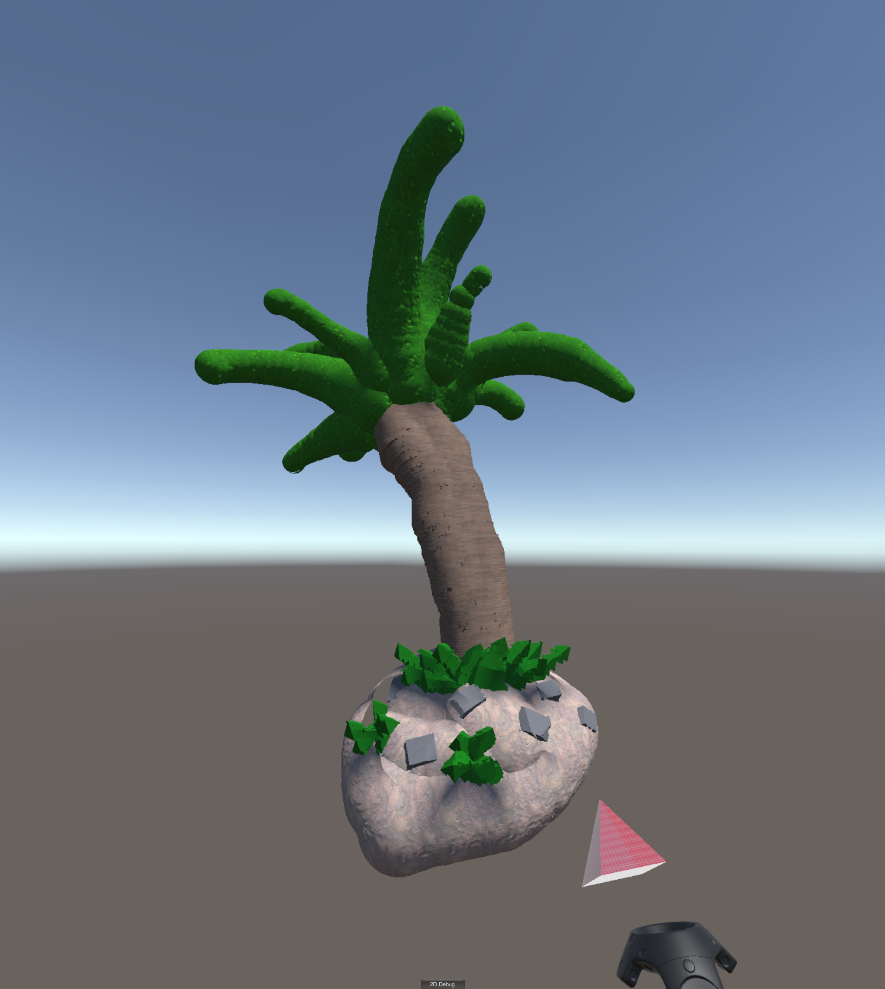
\includegraphics[width=\linewidth]{tree_sculpture.png}
\caption{A tree sculpture made in our VR sculpting application.}
\label{fig:tree_sculpture}
\endminipage\hfill
\end{figure}

\newpage

\section{User Evaluation Questionnaire}

% PDF stuff
\ifx\pdfoutput\undefined
\else
    \pdfpagewidth=210mm
    \pdfpageheight=297mm
\fi

\newif\ifbanner\bannerfalse
\bannerfalse
\advance\oddsidemargin-5mm
\advance\textwidth1cm

\font\manual=manfnt
\def\shared{\noindent\llap{\manual\char'170\kern.15em}}

\def\heading#1{
    \ifhmode\par\fi
    \removelastskip
    \vskip1ex plus 0.5ex minus 0.3 ex%\goodbreak
    \noindent
    \hbox to \hsize{ #1\hfill}
    \smallskip\par\nobreak}


\def\nicefrac#1/#2{\leavevmode%
    \raise.5ex\hbox{\the\scriptfont0 #1}%
    \kern-.1em/\kern-.15em%
    \lower.25ex\hbox{\the\scriptfont0 #2}}

\newdimen\scalewidth
\scalewidth=0.3\hsize 

\def\xboxit#1{\hbox{\lower0.7ex\vbox{\hrule\hbox{\vrule\kern1pt
    \vbox{\kern1pt\hbox{\strut\small #1}\kern1pt}\kern1pt\vrule}\hrule}}}

\def\boxit#1{\hbox{\lower0.7ex\vbox{\hrule\hbox{\vrule\kern1pt
    \vbox{\kern1pt\hbox to 1.4em
    {\small\strut\hfil #1\hfil}\kern1pt}\kern1pt\vrule}\hrule}}}

\def\sboxit{\hbox{\lower0.7ex\vbox{\hrule\hbox{\vrule\kern1pt
    \vbox{\kern1pt\hbox to 1ex
    {\small\strut\hfil}\kern1pt}\kern1pt\vrule}\hrule}}}


\def\fiveboxes#1#2#3#4#5{\hbox to\scalewidth
    {\boxit{#1}\hfil\boxit{#2}\hfil\boxit{#3}\hfil%
     \boxit{#4}\hfil\boxit{#5}}}
\def\manyboxes{\hbox to \scalewidth
    {\sboxit\hfil\sboxit\hfil\sboxit\hfil\sboxit\hfil\sboxit\hfil%
    \sboxit\hfil\sboxit\hfil\sboxit\hfil\sboxit\hfil\sboxit\hfil\sboxit}}


\def\boxes{\fiveboxes{}{}{}{}{}\ignorespaces}

\def\void{\boxit{}}

\def\xscale#1#2{%
    \setbox0=\hbox{\boxes}%
    \setbox1=\hbox to \wd0{\small\strut\hfill #2 $\to$}%
    \setbox2=\hbox to \wd0{\small\strut $\gets$ #1 \hfill}%
    \vbox{\vbox to 0pt{\vss\box1\box2\kern2pt}\vbox{\box0}}}

\def\scale#1#2{%
    \setbox0=\hbox{\boxes}%
    \setbox1=\hbox to \wd0{\small\strut\hfill #2 $\to$}%
    \setbox2=\hbox to \wd0{\small\strut $\gets$ #1 \hfill}%
    \vbox{\medskip\box1\box2\kern2pt\box0}}

\def\xshortscale#1#2{%
    \setbox0=\hbox{\boxes}%
    \setbox1=\hbox to \wd0{\small\strut $\gets$ #1 \hfill #2 $\to$}%
    \vbox{\vbox to 0pt{\vss\box1\kern2pt}\vbox{\box0}}}

\def\shortscale#1#2{%
    \setbox0=\hbox{\boxes}%
    \setbox1=\hbox to \wd0{\small\strut $\gets$ #1 \hfill #2 $\to$}%
    \vbox{\medskip\box1\kern2pt\box0}}

\def\agree{\scale{strongly disagree}{agree completely}}
\def\xagree{\xscale{strongly disagree}{agree completely}}
\def\xquality{\xshortscale{poor}{outstanding}}
\def\quality{\shortscale{poor}{outstanding}}

\def\longquality{%
    \setbox0=\hbox{\manyboxes}%
    \setbox1=\hbox to \wd0{\small\strut $\gets$ poor \hfill outstanding $\to$}%
    \vbox{\vbox to 0pt{\vss\box1\kern2pt}\vbox{\box0}}}

\def\linscale{%
    \def\tick{\vrule height 5pt\relax}%
    \vbox{\hbox to \scalewidth{\tick\hfil\tick\hfil\tick\hfil\tick}\hrule}}

\def\question#1\par#2\par{\hbox to \hsize
    {\vbox{\hsize=0.72\hsize #1\dotfill}\quad#2\hfil}\medskip\goodbreak}

\def\freequestion#1\par{#1\par\nobreak
    \begingroup\nobreak
    \advance\leftskip by 2pc
    \hrule width 0pt height 1.7\baselineskip\hrulefill
    \hrule width 0pt height 1.7\baselineskip\hrulefill
    \par
    \medskip
    \endgroup
    }
		
\def\longfreequestion#1\par{#1\par\nobreak
    \begingroup\nobreak
    \advance\leftskip by 2pc
    \hrule width 0pt height 1.7\baselineskip\hrulefill
    \hrule width 0pt height 1.7\baselineskip\hrulefill
    \hrule width 0pt height 1.7\baselineskip\hrulefill
    \hrule width 0pt height 1.7\baselineskip\hrulefill
    \hrule width 0pt height 1.7\baselineskip\hrulefill
    \hrule width 0pt height 1.7\baselineskip\hrulefill
    \hrule width 0pt height 1.7\baselineskip\hrulefill
    \hrule width 0pt height 1.7\baselineskip\hrulefill
    \par
    \medskip
    \endgroup
    }

\parindent0pt
\parskip5pt plus 0.2 ex minus 0.1ex


\def\<#1>{\textsc{#1}}
\parindent0pt
\parskip5pt plus 0.2 ex minus 0.1ex

%\begin{document} 

The purpose of this user evaluation is to gather insight and feedback about the current implementation
of the sculpting and querying functionality and the impression it has on users. The results will be
helpful in identifying shortcomings and to improve the user experience.\\ \hfill
If at any point you feel unwell or nauseous while using the VR headset please let me know. That can be a common reaction when not used
to VR or when the program is not responsive enough.\\ \hfill
Each time before moving on a next task please press the "! Reset Scene !" button in the ingame "Query \& Utilities Menu" to reset the scene.


\newcounter{questionnumber}

\hfill \break
\heading{\textbf{Background}}

1: not at all, 2: slighty, 3: moderately, 4: very, 5: extremely \newline


\fbox{\begin{minipage}{1.05\linewidth}
\begin{minipage}{0.95\linewidth}
\question \stepcounter{questionnumber} \textbf{\arabic{questionnumber}.} How experienced are you with Virtual Reality? \par \fiveboxes{\color{gray}1}{\color{gray}2}{\color{gray}3}{\color{gray}4}{\color{gray}5} \par
\end{minipage}
\end{minipage}}


\fbox{\begin{minipage}{1.05\linewidth}
\begin{minipage}{0.95\linewidth}
\question \stepcounter{questionnumber} \textbf{\arabic{questionnumber}.} How experienced are you with 3D sculpting applications? \par \fiveboxes{\color{gray}1}{\color{gray}2}{\color{gray}3}{\color{gray}4}{\color{gray}5} \par
\end{minipage}
\end{minipage}}

\newpage
\heading{\textbf{Sculpting}}

1: very easy, 2: easy, 3: neutral, 4: difficult, 5: very difficult \newline

\fbox{\begin{minipage}{1.05\linewidth}
\begin{minipage}{0.95\linewidth}
\question \stepcounter{questionnumber} \textbf{\arabic{questionnumber}.}
Read the controller hints to become familiar with VR and the control scheme. Disable the controller hints once you're ready. Please note that you can activate these hints
again at any time if necessary.\\ \hfill
Time limit: 5min.
\par \fiveboxes{\color{gray}1}{\color{gray}2}{\color{gray}3}{\color{gray}4}{\color{gray}5}

\freequestion Feedback: \par
\end{minipage}
\end{minipage}}


\fbox{\begin{minipage}{1.05\linewidth}
\begin{minipage}{0.95\linewidth}
\question \stepcounter{questionnumber} \textbf{\arabic{questionnumber}.}
Select the sphere brush and place it the world to create a shape or simple sculpture using the 'Add' mode.\\ \hfill
Time limit: 5min.
\par \fiveboxes{\color{gray}1}{\color{gray}2}{\color{gray}3}{\color{gray}4}{\color{gray}5}

\freequestion Feedback: \par
\end{minipage}
\end{minipage}}


\fbox{\begin{minipage}{1.05\linewidth}
\begin{minipage}{0.95\linewidth}
\question \stepcounter{questionnumber} \textbf{\arabic{questionnumber}.}
Select a brush and create a shape, then select another brush and remove a piece of your sculpture with it using the 'Remove' mode.\\ \hfill
Time limit: 5min.
\par \fiveboxes{\color{gray}1}{\color{gray}2}{\color{gray}3}{\color{gray}4}{\color{gray}5}

\freequestion Feedback: \par
\end{minipage}
\end{minipage}}


\fbox{\begin{minipage}{1.05\linewidth}
\begin{minipage}{0.95\linewidth}
\question \stepcounter{questionnumber} \textbf{\arabic{questionnumber}.}
Select a brush and create a shape, then pick another colour and colour a piece of your sculpture using the 'Replace' mode.\\ \hfill
Time limit: 5min.
\par \fiveboxes{\color{gray}1}{\color{gray}2}{\color{gray}3}{\color{gray}4}{\color{gray}5}

\freequestion Feedback: \par
\end{minipage}
\end{minipage}}


\fbox{\begin{minipage}{1.05\linewidth}
\begin{minipage}{0.95\linewidth}
\question \stepcounter{questionnumber} \textbf{\arabic{questionnumber}.}
Select a brush and create a shape, then pick another material (i.e. texture) and change the material of a piece of your sculpture using the 'Replace' mode.\\ \hfill
Time limit: 5min.
\par \fiveboxes{\color{gray}1}{\color{gray}2}{\color{gray}3}{\color{gray}4}{\color{gray}5}

\freequestion Feedback: \par
\end{minipage}
\end{minipage}}


\fbox{\begin{minipage}{1.05\linewidth}
\begin{minipage}{0.95\linewidth}
\question \stepcounter{questionnumber} \textbf{\arabic{questionnumber}.}
Create your own brush (with at least two primitives) using the custom brush editor and then use your own brush to create a shape.\\ \hfill
Time limit: 8min.
\par \fiveboxes{\color{gray}1}{\color{gray}2}{\color{gray}3}{\color{gray}4}{\color{gray}5}

\freequestion Feedback: \par
\end{minipage}
\end{minipage}}


\hfill \break
\heading{\textbf{Querying}}

1: very easy, 2: easy, 3: neutral, 4: difficult, 5: very difficult \newline


\fbox{\begin{minipage}{1.05\linewidth}
\begin{minipage}{0.95\linewidth}
\question \stepcounter{questionnumber} \textbf{\arabic{questionnumber}.}
Select a brush and create a shape, then use the query menu to run a similarity search.\\ \hfill
Time limit: 6min.
\par \fiveboxes{\color{gray}1}{\color{gray}2}{\color{gray}3}{\color{gray}4}{\color{gray}5}

\freequestion Feedback: \par
\end{minipage}
\end{minipage}}


\fbox{\begin{minipage}{1.05\linewidth}
\begin{minipage}{0.95\linewidth}
\question \stepcounter{questionnumber} \textbf{\arabic{questionnumber}.}
Select a brush and create a shape, then use the query menu to run a similarity search. After that, pick one of the results and voxelize it into the world.\\ \hfill
Time limit: 6min.
\par \fiveboxes{\color{gray}1}{\color{gray}2}{\color{gray}3}{\color{gray}4}{\color{gray}5}

\freequestion Feedback: \par
\end{minipage}
\end{minipage}}


\fbox{\begin{minipage}{1.05\linewidth}
\begin{minipage}{0.95\linewidth}
\question \stepcounter{questionnumber} \textbf{\arabic{questionnumber}.}
Select a brush and create a shape, then use the query menu to run a similarity search. After that, pick one of the results and voxelize it. Using a brush, remove a piece of it and then run a similarity search for the modified sculpture.\\ \hfill
Time limit: 8min.
\par \fiveboxes{\color{gray}1}{\color{gray}2}{\color{gray}3}{\color{gray}4}{\color{gray}5}

\freequestion Feedback: \par
\end{minipage}
\end{minipage}}


\fbox{\begin{minipage}{1.05\linewidth}
\begin{minipage}{0.95\linewidth}
\stepcounter{questionnumber} \textbf{\arabic{questionnumber}.}
That was all, thank you! If you feel like playing around some more with the program feel free to do so for a couple more minutes.
On the next page you can give general feedback.\\ \hfill
Time limit: 5min.
\end{minipage}
\end{minipage}}


\heading{\textbf{General feedback}}

\fbox{\begin{minipage}{1.05\linewidth}
\begin{minipage}{0.95\linewidth}
\longfreequestion \stepcounter{questionnumber} \textbf{\arabic{questionnumber}.} If you have any additional remarks or suggestions for improvements please write them down here. \par
\end{minipage}
\end{minipage}}



\newpage